%%%%%%%%%%%%%%%%%%%%%%%%%%%%%%%%%%%%%%%%%%%%%%
\section{Beam plug}
\label{sec:beamplug}
\fixme{Rearrange the text so beam plug is described here. The beam window penetration through the cryostat insulation layers is described in the crystat section}
The charged particles from the H4 beamline will first need to go through the cryostat insulation layers before reaching the inside of the cryostat. After which the particle beam will still need to penetrate another $\approx$45~cm of passive LAr layer and the field cage before entering the active TPC region. In order to allow the particle beam to enter the TPC with minimal energy loss and multiple scattering from upstream materials, a beam window penetration is inserted into the crystat insulation layers (described in Section~\ref{subsec:beamwindow}) and a beam plug is installed inside the cryostat along the beam path. The beam plug design is described in this section.

%
%%%%%%%%%%%%%%%%%%%%%%%%%%%%
%Remove System 1 discussion
%%%%%%%%%%%%%%%%%%%%%%%%%%%
%The main function of the beam window system is to allow charged particles from the H4 beam line to enter the TPC with minimal energy loss and multiple scattering. The system penetrates through the cryostat insulation layers, displaces approximately 45cm of passive LAr layer, and extends inside the active TPC region through an opening in the TPC field cage. To keep the primary stainless steel membrane of the cryostat intact, the beam window is divided into two independent subsystems. The first system (system 1) is installed inside the cryostat insulation layer and ends at the primary cryostat membrane. The second system (system 2) is inside the LAr portion of the cryostat. For NP04, the H4 beam line is designed to be able to inject beam into the LAr cryostat at three different locations. Due to various engineering and safety constraints, only one of the beam injection points will have the full beam window system installed. The sketch of the beam window system is shown in Figure~\ref{fig:beamwindow_fig1}. The details of the design are described in the following sections.
%\begin{cdrfigure}[Beam window systems]{beamwindow_fig1}{Beam window system 1 and 2.}
%  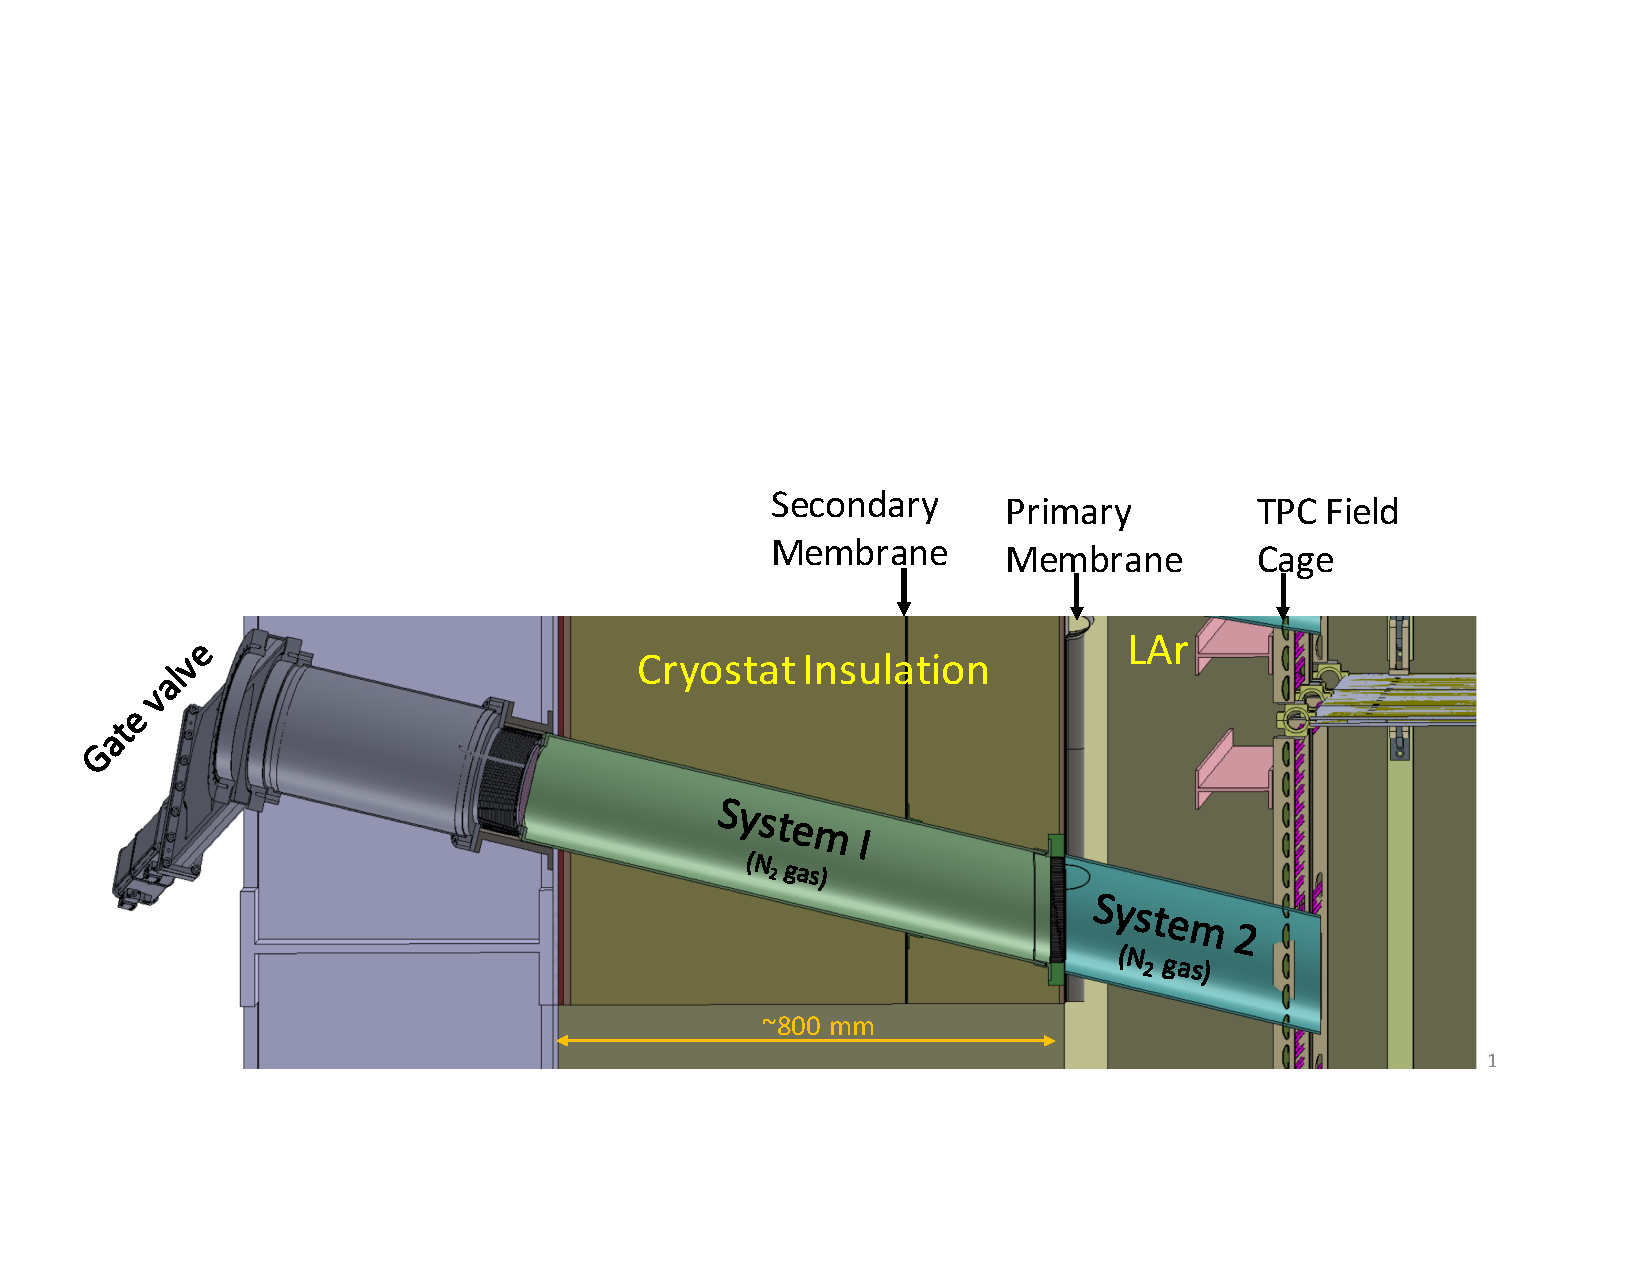
\includegraphics[width=0.90\textwidth]{beamwindow_system1and2.pdf}
%\end{cdrfigure}
%%%%%%%%%%%%%%%%%%%%%%%%%%%%
%Remove System 1 discussion
%%%%%%%%%%%%%%%%%%%%%%%%%%%
%\subsection{System 1}
%A close-up view of the System 1 beam window is shown in Figure~\ref{fig:beamwindow_zoom}. The system 1 beam window is a cylindrical G10 (OD$\approx$22cm) tube with a nomex honeycomb core at each end. The tube is filled with dry nitrogen gas and maintained at about 1 atm of pressure. It is designed to provide thermal insulation with a heat load of less than 5W/$m^2$. As shown in Figure~\ref{fig:beamwindow_fig1}, system 1 beam window extends to the external steel support structure of the cryostat. The other end of the beam window is in physical contact with the cryostat's primary membrane. When the cryostat is filled with LAr, the nomex honeycomb core provides the structural support to prevent the membrane from bulging outward. The honeycomb core on the other end of the tube, where the bellow is located, provides thermal insulation to keep ice from building up on the outer surface. The secondary membrane will be bonded onto a cylindrical disk attached to the G10 shell during installation. The system 1 beam window is anchored to the outer steel structure of the cryostat with a flange. As an additional safety measure, there is an option to install a gate valve on the external end of the beam window.
%\begin{cdrfigure}[Beam window 1 zoomed]{beamwindow_zoom}{A detailed view of system 1 beam widnow.}
%  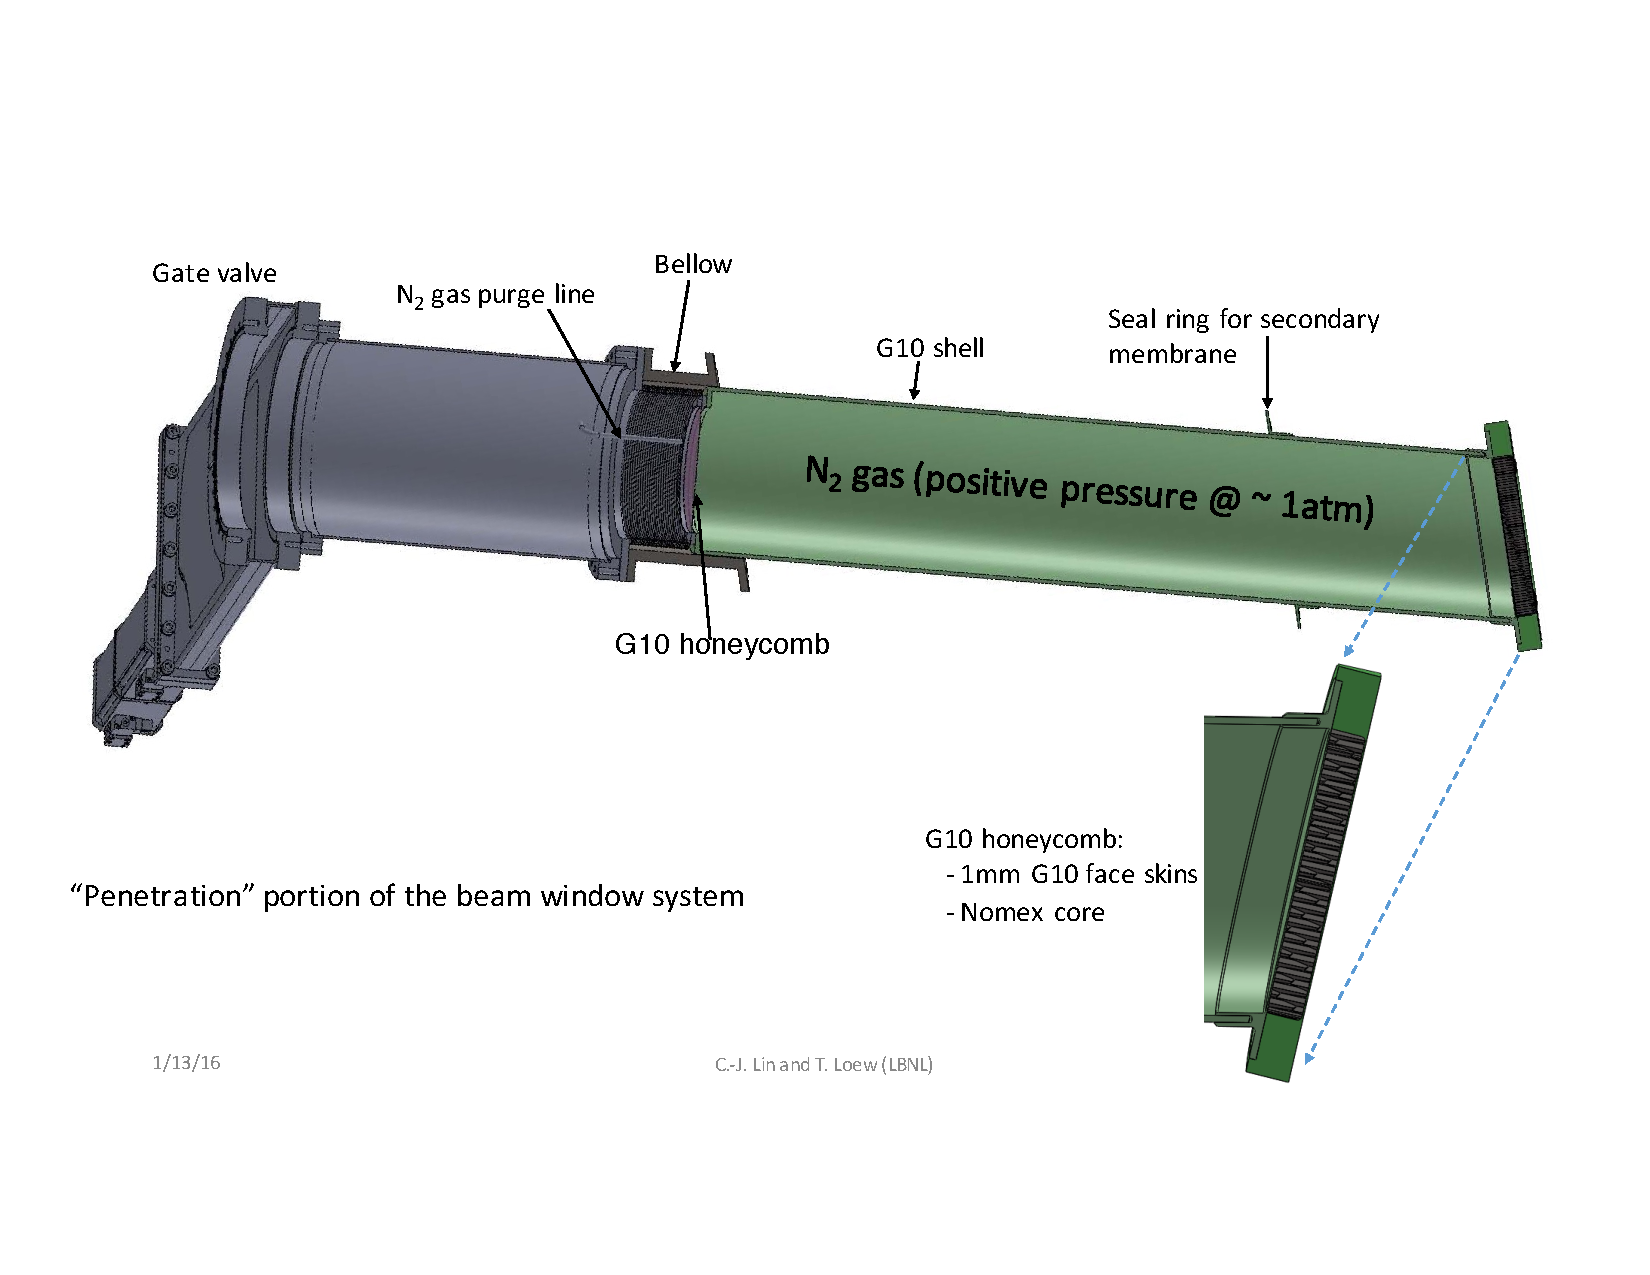
\includegraphics[width=0.90\textwidth]{beamwindow_system1zoom.pdf}
%\end{cdrfigure}

The beam plug is designed to displace the passive LAr layer between the TPC field cage and the inner crystat membrane. As illustrated in Figure~\ref{fig:beamwindow_fig2}, it is a cylidrical glass-fiber composite pressure vessel about 50cm in length and  22cm in diameter. It is filled with dry nitrogen gas via a stainless steel line that extends to the top of the cryostat. The pressure inside the beam plug is maintained externally to about 25 psi from room to LAr temperatures. A pressure relief valve (or burst disk) will be installed on the nitrogen fill line on the top of the cryostat (externally) to ensure the pressure inside the beam plug does not exceed the safety level. The component-level view of the beam plug is shown in Figure~\ref{fig:beamplug_components}.  The beam plug is secured to the field cage support structure (see Section~\ref{subsec:fc-beamplug}). The front portion of the beam plug extends about 5~cm inside the field cage through an opening on the field cage. The field cage support is designed with sufficient strength to withstand the weight of the beam plug while it is suspended in air. When the cryostat is filled with LAr, the beam plug is roughly neutrally buoyant. 

At nominal operation, the voltage difference across the beam plug could be as high as 165kV. To minimize electrical discharges, the beam plug is divided into sections and each section is bonded to a stainless steel conductive grading rings. The grading rings are conected in series with two parallel path of resistor chains. There are 7 grading rings. The ring that is closest to the field cage is electrically connected to one of the field cage profiles. The last ring near the cryostat wall is grounded to the stainless steel membrane. The type and value of the resistor is still under evaluation. A likely candidate is the high voltage Super Mox 15G$\Omega$ resistor by OHMITE. The maximum total power dissipated by the resistor chain is about 0.6W.

\begin{cdrfigure}[Beam plug]{beamwindow_fig2}{Beam plug. It is a  composite pressure vessel filled with dry nitrogen gas. The vessel is about 50cm in length and about 22cm in diameter. The pressure vessel is divided into sections with each section bonded to a stainless steel grading ring. The grading rings are connected by two parallel paths of resistor chain.}
  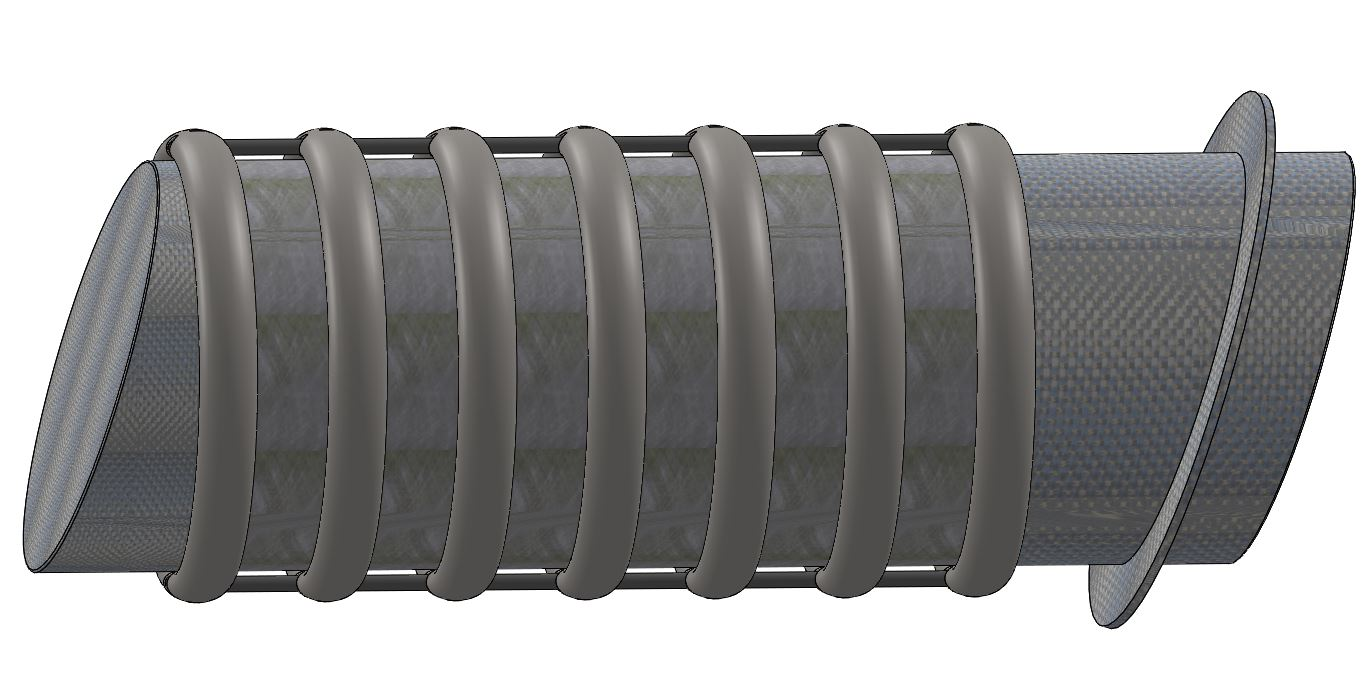
\includegraphics[width=0.65\textwidth]{beamwindow_system2.jpg}
\end{cdrfigure}

\begin{cdrfigure}[Beam plug component-level view]{beamplug_components}{Component-level view of the beam plug showing alternating electrode and composite ring structure.}
  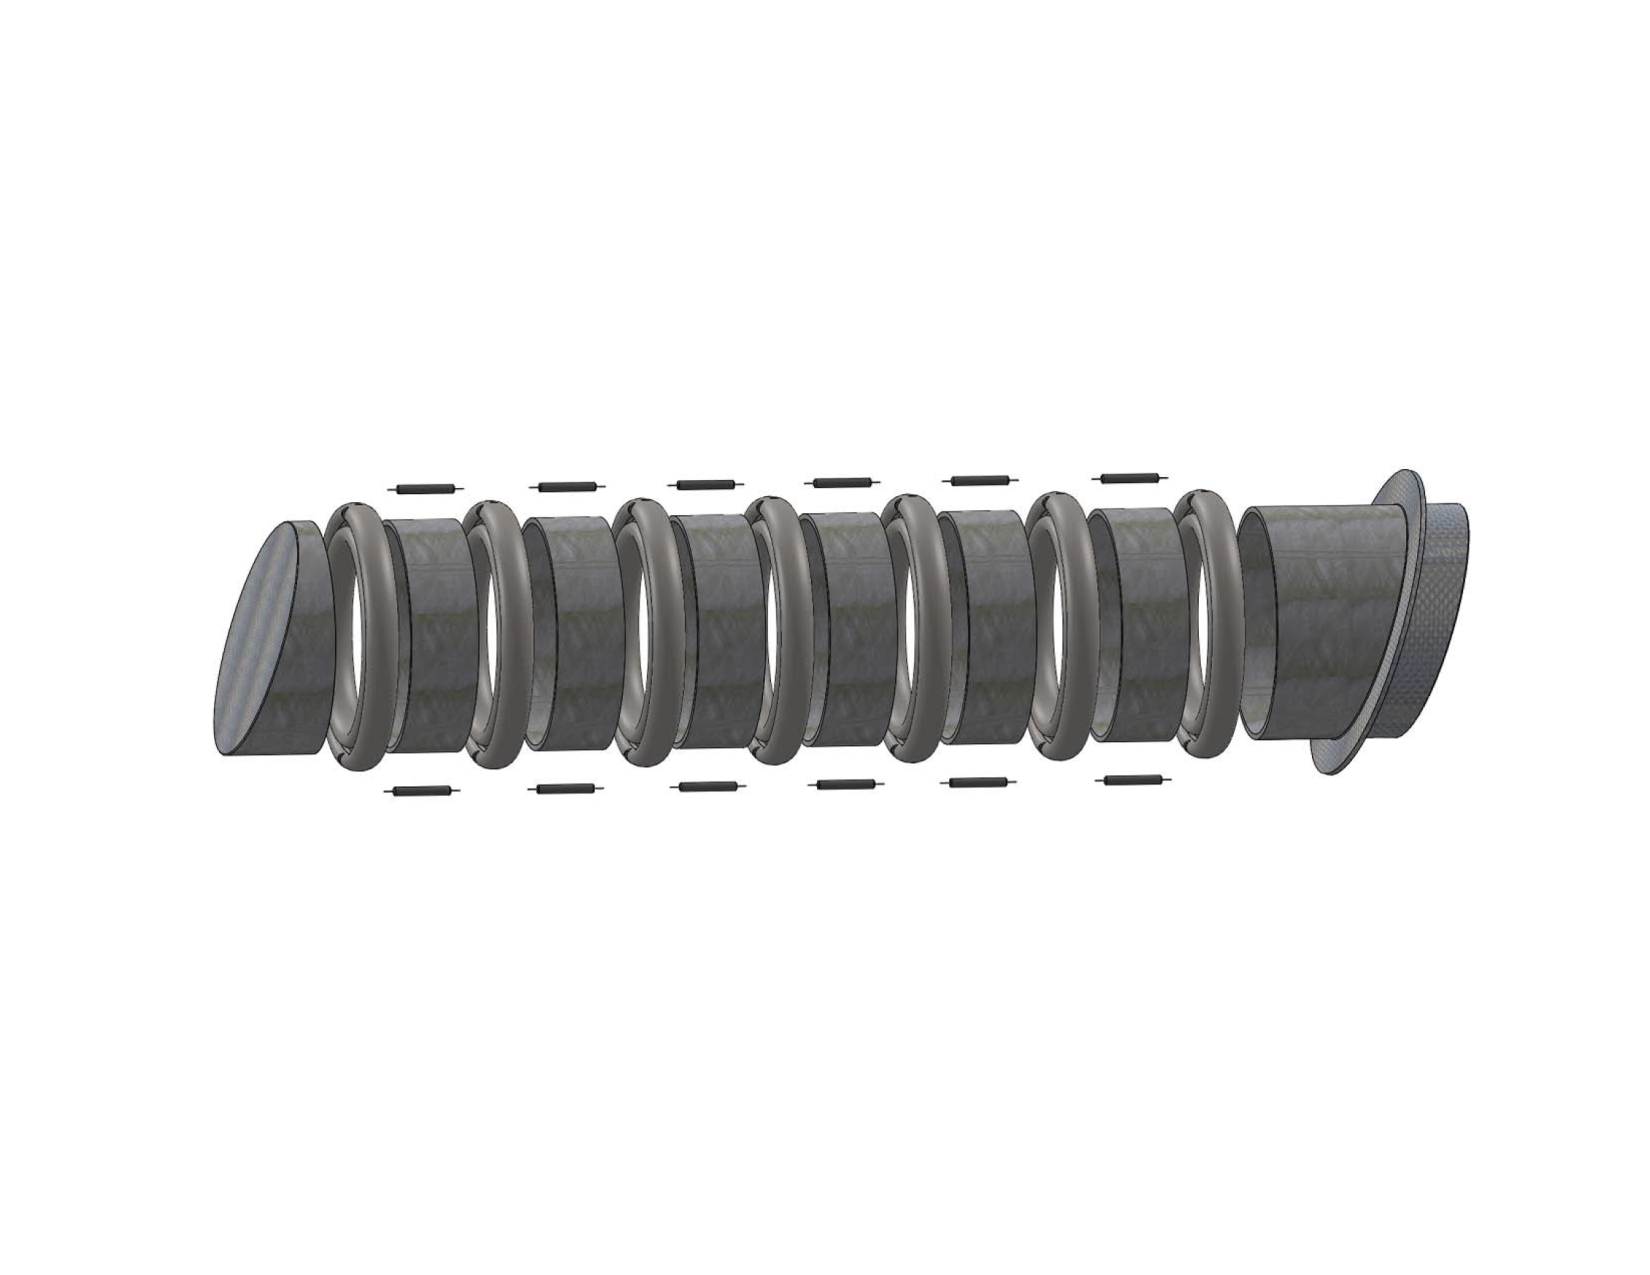
\includegraphics[width=0.90\textwidth]{beamplug_components.pdf}
\end{cdrfigure}

\subsection{Adhesive shear testing of ring joints}
The stainless steel electrodes and the composite shells will be bonded using a cryogenically rated epoxy system (Hysol 9309.2 NA). The vendor has fabricated prototype pieces to measure the adhesive shear strength for the proposed joints. The measurements were done at cryogenic temperature and also as a function of bond length. Testing results indicate that the default design has at least a safety factor of 6 for axial adhesive shear failure. The test samples and setup are shown in Figure~\ref{fig:beamplug_sheartest}.

\begin{cdrfigure}[Beam plug Shear Test]{beamplug_sheartest}{Photo on the left shows the bonded test samples. The measurements were performed for different bond lengths and componsite shell thicknesses. Photo on the right shows the test setup. The tests were done at LN temperature.}
  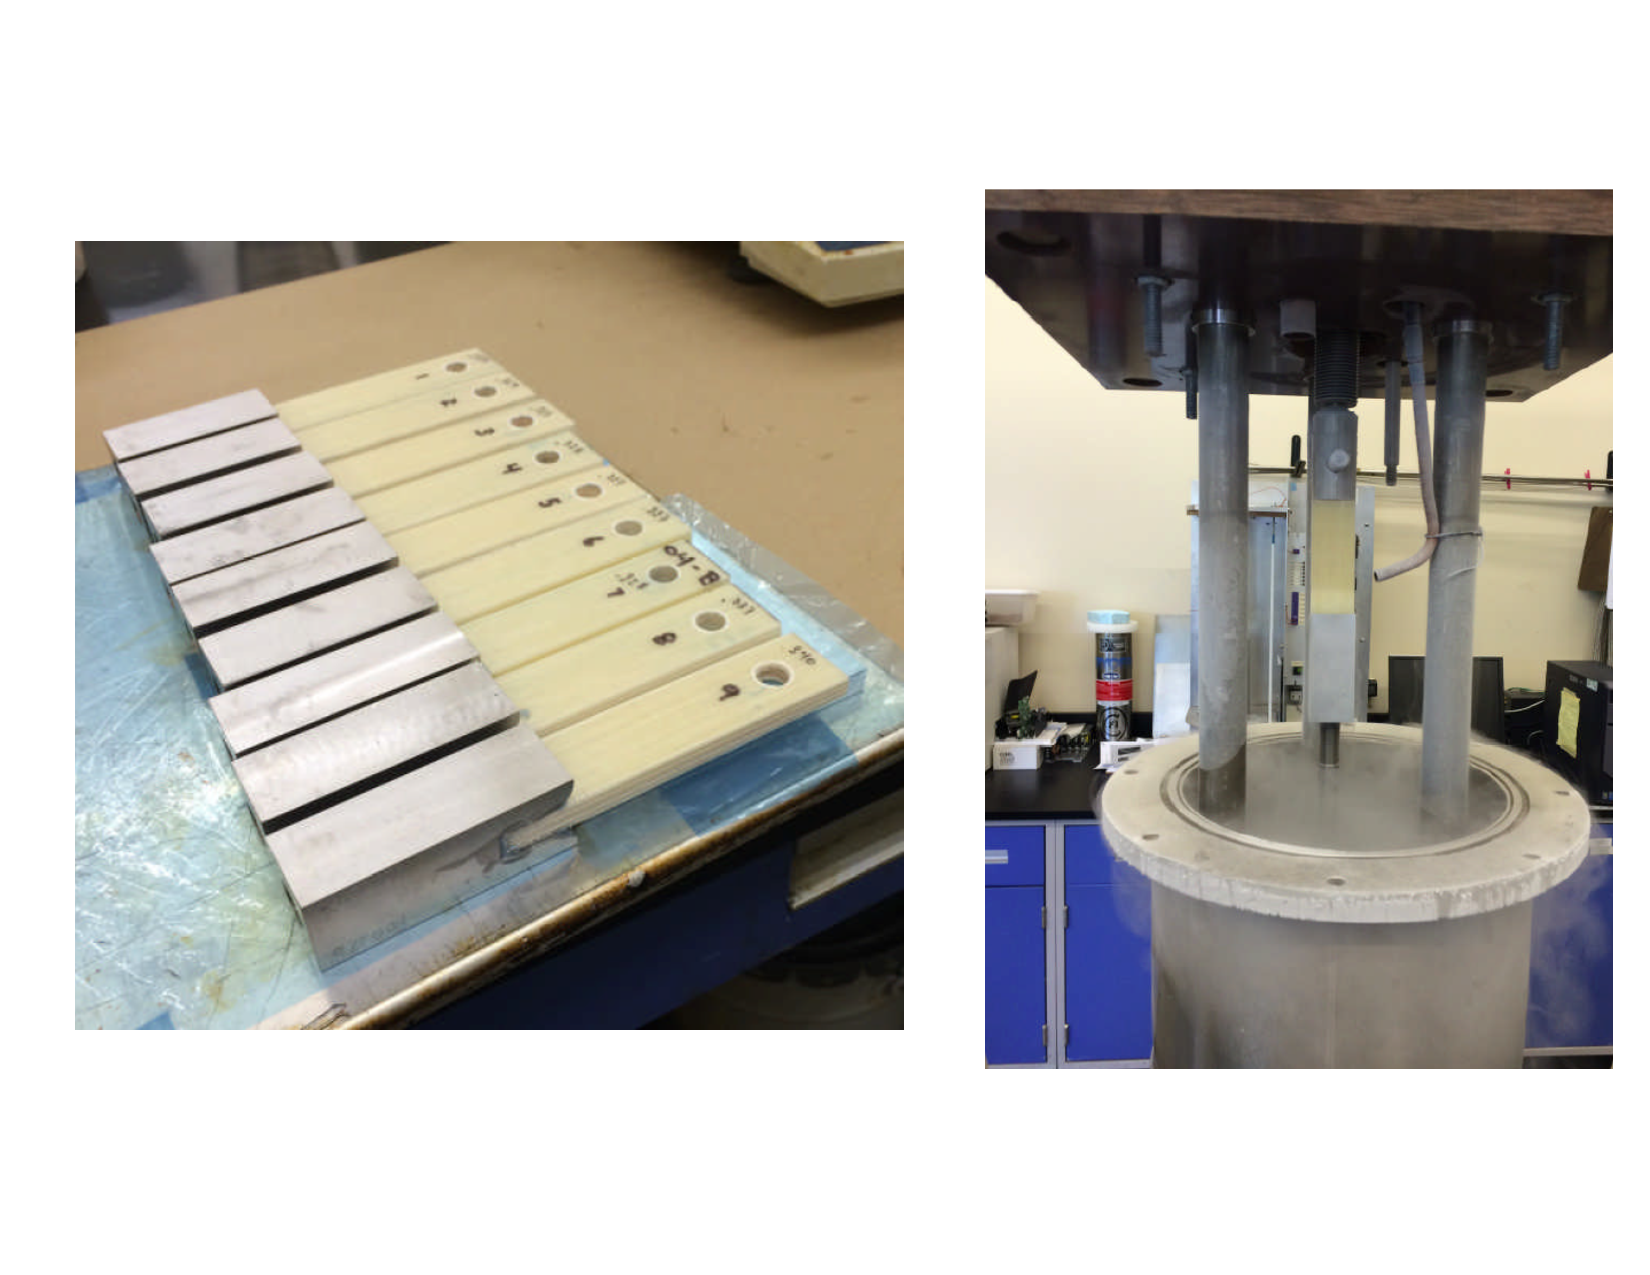
\includegraphics[width=0.85\textwidth]{beamplug_sheartest.pdf}
\end{cdrfigure}


\subsection{Electrode ring design}
The metal electrode rings are spaced at regular intervals and interspersed with composite tube sections. The shape of the rings has been designed to minimize high electric field corners. The results of the field calculations are shown in Figures~\ref{fig:beamplug_ring1} and~\ref{fig:beamplug_ring2}. The average field in the vicinity of the beam plug is about 4.4 kV/cm. The maximum field of 15.7 kV/cm is on the electrode ring surface. The field at all region is well below the 30 kV/cm limit.

\begin{cdrfigure}[Beam plug electrodes]{beamplug_ring1}{Electric field calculation of the electrode ring design. The average field in the beam plug region is about 4.4 kV/cm. The maximum field of 15.7 kV/cm is on the electrode ring surface. }
  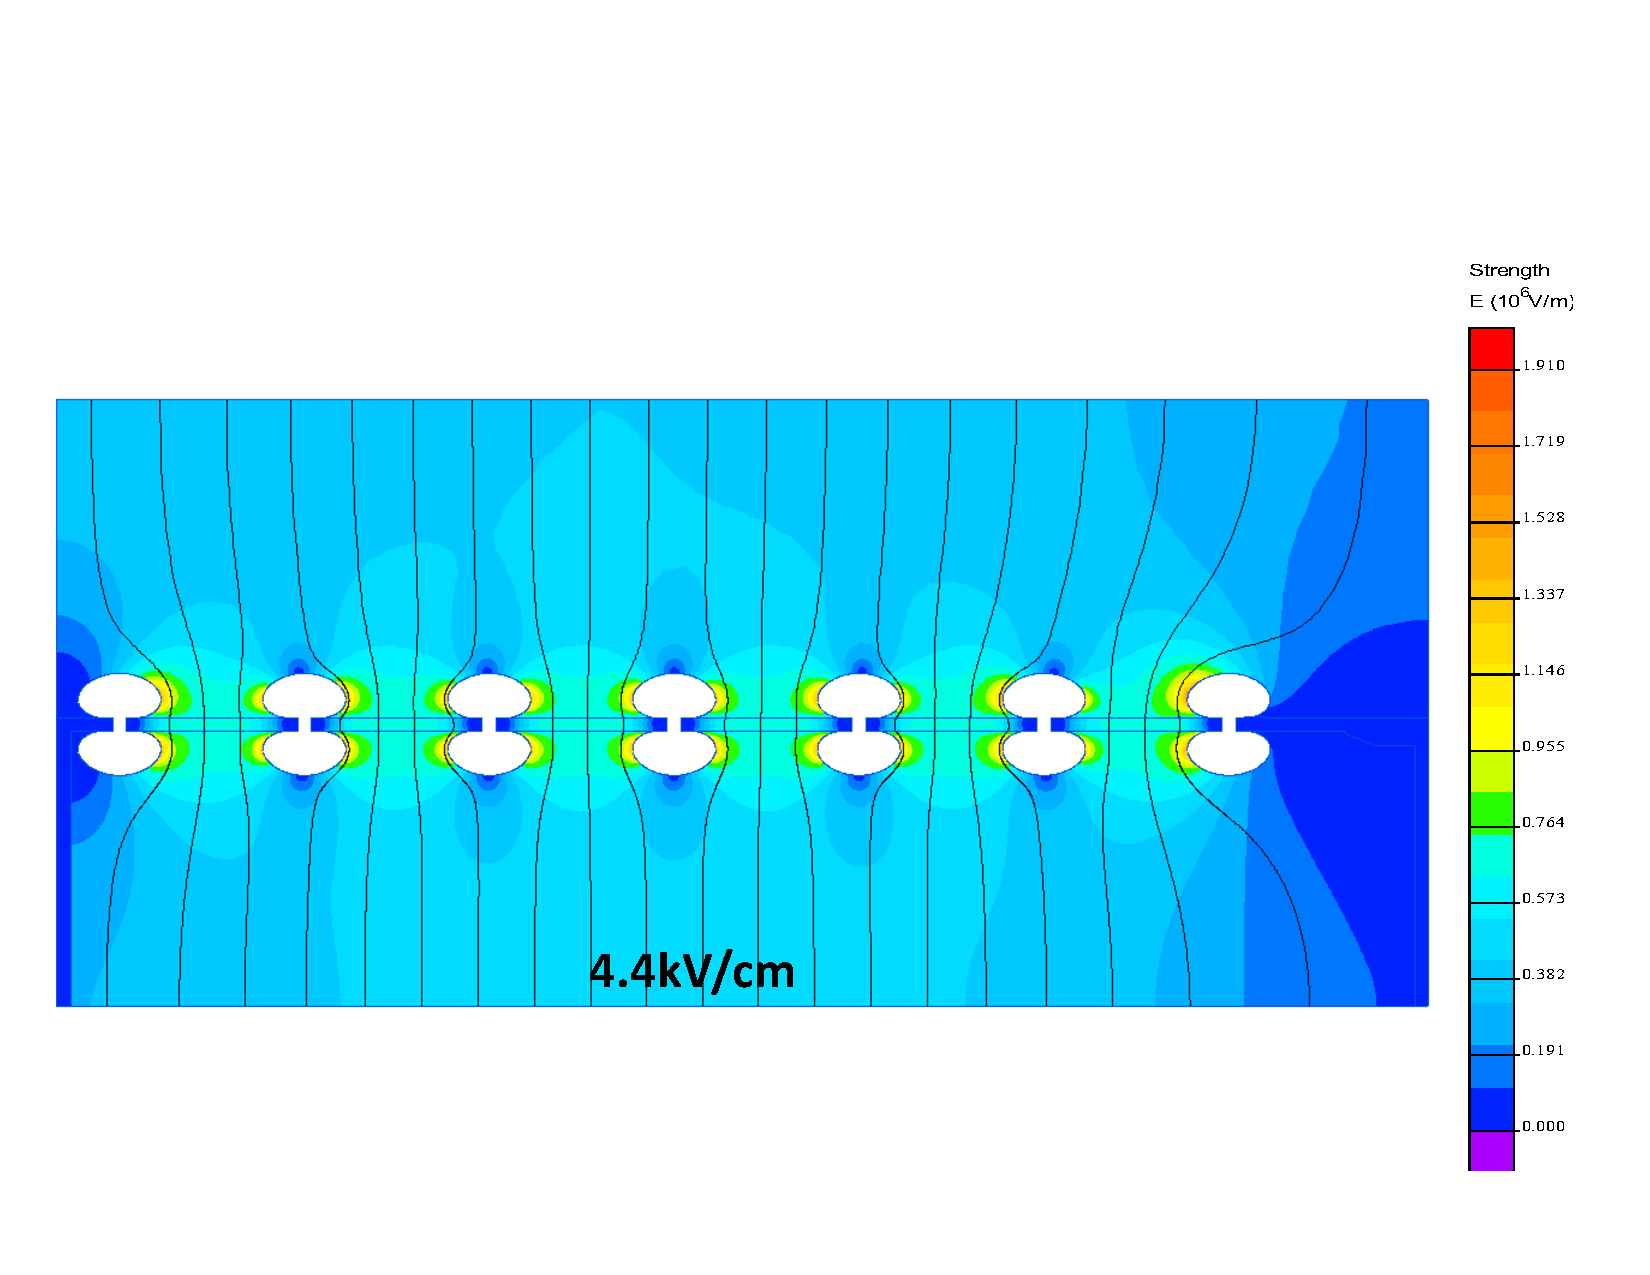
\includegraphics[width=0.85\textwidth]{beamplug_ring1.pdf}
\end{cdrfigure}

\begin{cdrfigure}[Beam plug electrode]{beamplug_ring2}{Electric field calculation near the vicinity of the electrode. The shape of the ring minimizes the high field region near the joints between the electrode, LAr, and composite shell. The field at all region is well below the 30 kV/cm limit.}
  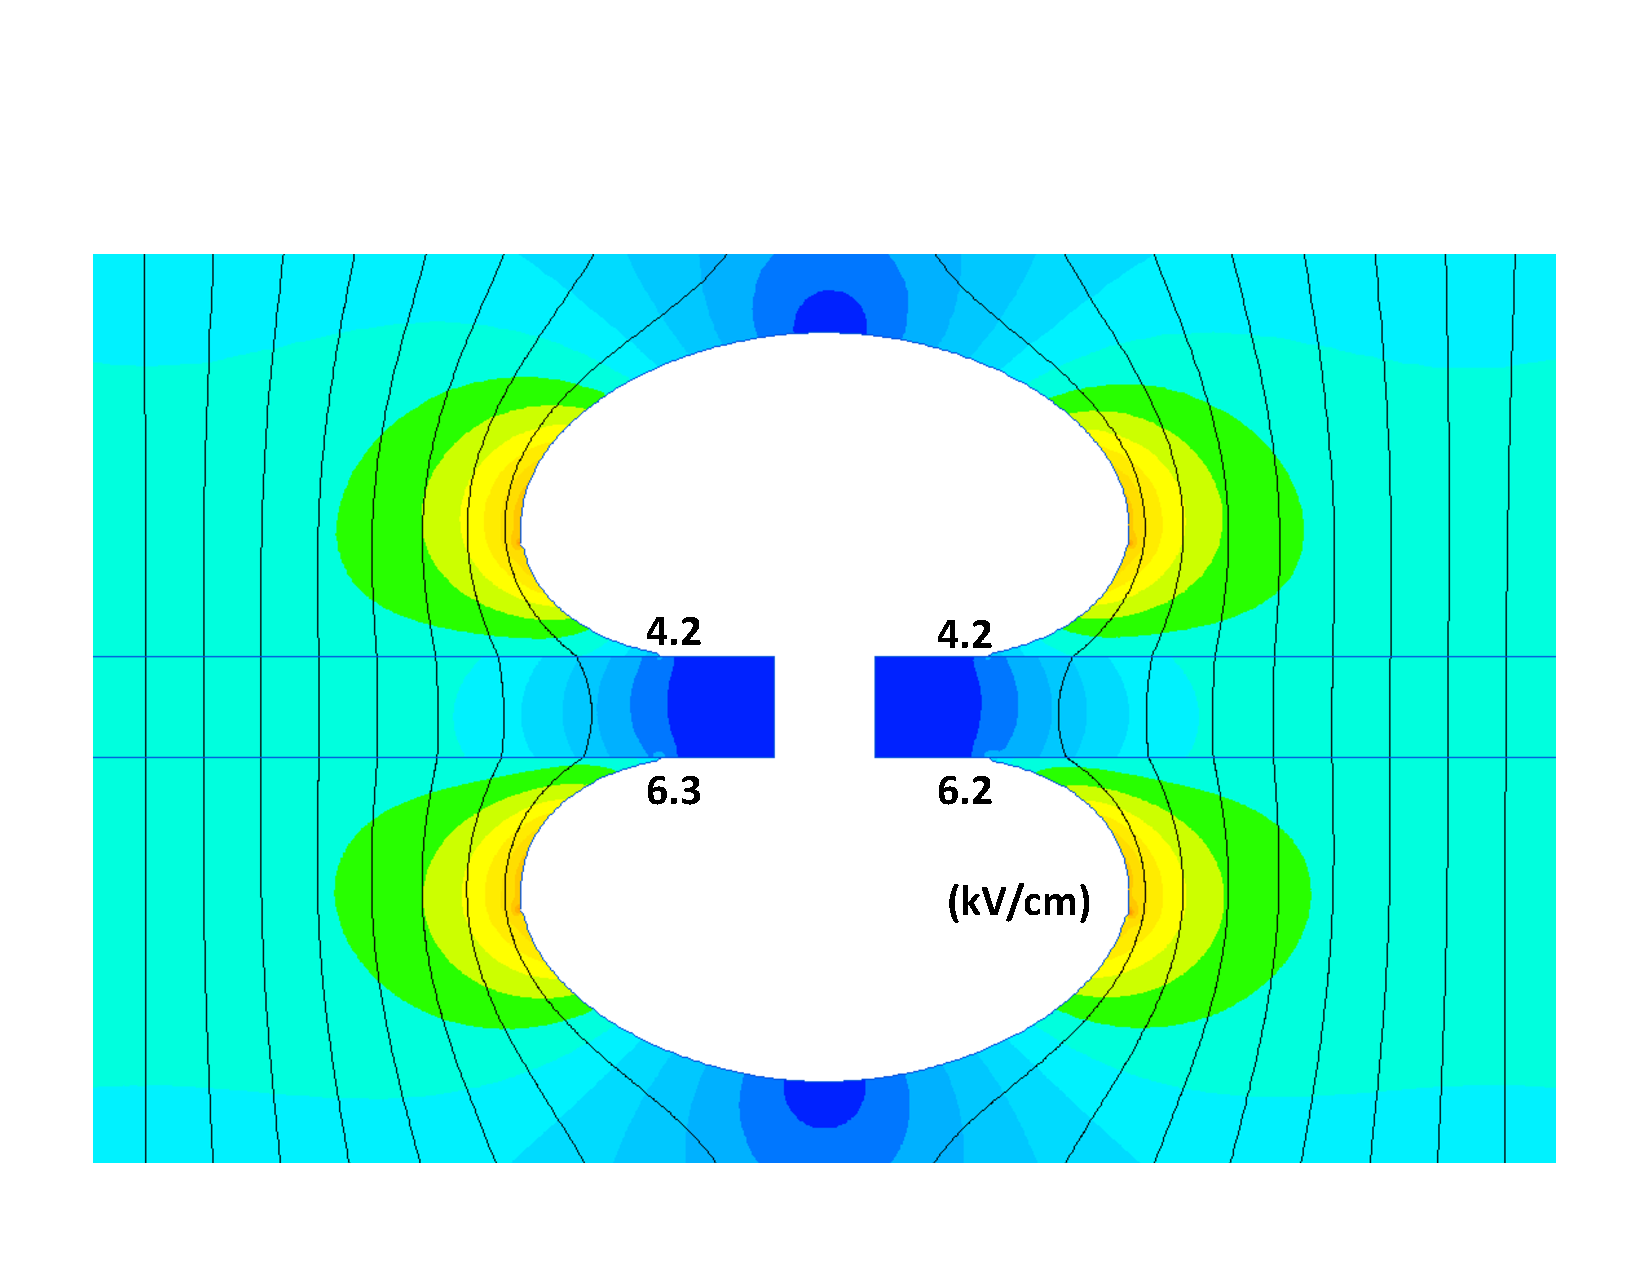
\includegraphics[width=0.65\textwidth]{beamplug_ring2.pdf}
\end{cdrfigure}

\subsection{Dielectric strength of composite shell}

\begin{cdrfigure}[Dielectric strength test]{beamplug_dielectric}{Test setup to measure the dielectric breakdown of the composite material. The sample tested is shown in the photo on the left. The composite plate is attached to the electrodes that have been machined to match the geometry of the beam plug. The photo on the right shows the HV connection.}
  \includegraphics[width=0.85\textwidth]{beamplug_dielectric.pdf}
\end{cdrfigure}



\begin{cdrtable}[Beam plug requirements]{lll}{bprequirements}{Beam plug requirements and parameters list}
Parameter & Value & Notes \\ \toprowrule
Dimensions & & Defined by CAD model \\ 
~~Internal Diameter (est) & 200~mm & At composite ring ID surface; \\
                          &        & tolerance for assembly \\ 
~~Wall thickness (est) & 8~mm & Tolerance for assembly \\ 
~~Length (est) & 495~mm $\pm$ 1~mm & Overall (Normal Distance) \\ 
               & 577~mm $\pm$ 1~mm & Overall (Absolute Distance) \\ \colhline 
Metal End Cap Angle & (16.2$\pm$0.25)$^\circ$ & From perpendicular; \\ 
                    &                         &maintain length tolerance \\ 
Composite End Cap   & (16.2$\pm$0.5)$^\circ$ & From perpendicular; \\ 
                    &                        & maintain length tolerance \\ 
Flange Angle        & (16.2$\pm$0.25)$^\circ$ & From perpendicular \\ \colhline 
Tolerances  & ASME Y14.5 2009 & Where useful to convey design intent \\
            &                 & and function \\ 
Materials used   & & Electrically insulating; selected from or\\
                 & & approved per FNAL LAr purity list \\ 
Epoxy system & Hysol 9309.2 NA & Rated for cryogenic use\\
Electrode Rings & 304 Stainless steel & \\ \colhline 
Resistor Type & OHMITE Super-Mox 930 Series & \\
Resistor Value & 15~G$\Omega$ & \\
Number of resistors & 6 & \\
Power dissipation &  &\\ 
~~Per resistor    & $\approx$0.1W & \\
~~Total           & $\approx$0.6W & \\ \colhline 
Operating Voltage & Up to 180 kV end-to-end & Electrically insulative \\ 
Operating Temperature & 25$^\circ$~C & Room temperature \\ 
                      & -185$^\circ$~C & LAr temperature \\ 
Operating Pressure    & 25~psi & MAWP at operating temperature \\ 
(Internal, External) && \\ \colhline 
Pressure Environment & 14.7 psi & Ambient temperature \\
(External)           & 19.9 psi & LAr temperature \\ \colhline
Internal Volume & 15.5 liter (est.) & Internal \\
                & 22 liter (est.) & External displacement \\ \colhline
Permeability/Leak Rate  & 7.8$\times$10$^{-5}$ scc/s to & He gas equivalent \\
Range                             & 15.6$\times$10$^{-5}$ scc/s \\ \colhline
Operating Lifetime   & 1 yr  &  \\
Lifetime Operational Thermal & 4 & \\
~Cycles to 77 K & & \\ \colhline
Shock Loading & & No design shock loading \\
Vibration Loading & & No design vibration loading \\ \colhline
Flange Profile & & Geometry per LBNL ICD \\
Weight (est.) & 75 lb [34 kg] & With SS304 electrode rings \\
Buoyancy Load (est.) & 67.5 lb [31 kg] & \\
Pressure Port & & Ground cap interface per LBNL \\ \colhline
Design Safety Factor & 2 & On MAWP (=50 psi) \\
Pressure Test Factor & 1.5 & Pneumatic test \\
High Voltage Tests & (180 kV equivalent) & \\ 
\end{cdrtable}


%\begin{cdrfigure}[System 2 beam window mounting scheme]{beamwindow_fig3}{System 2 beam window mounting scheme (preliminary). The beam plug is mounted to the field cage support structure.}
%  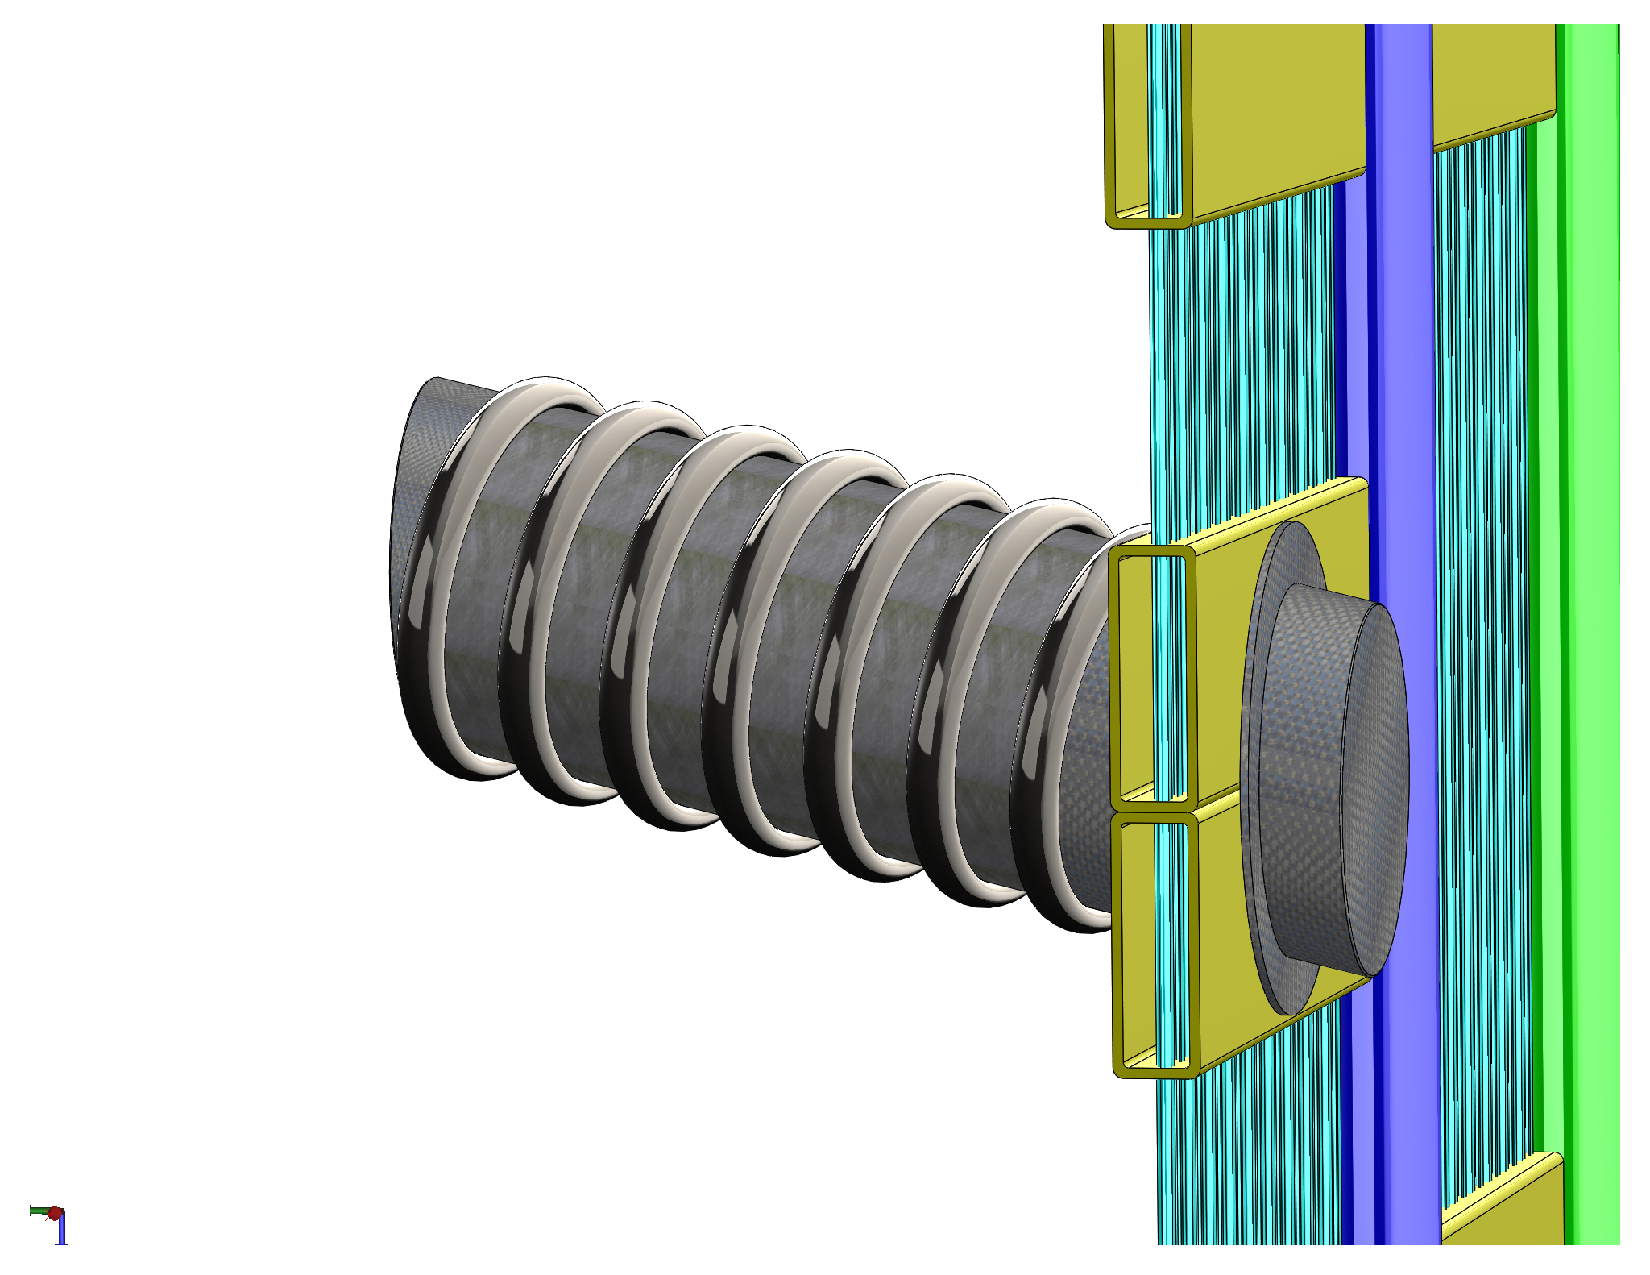
\includegraphics[width=0.7\textwidth,height=0.3\textheight]{beamwindow_system2_mount.pdf}
%\end{cdrfigure}



%%%%%%%%%%%%%%%%%%%%%%%%%
\subsection{QC Procedures}

\subsubsubsection{BLANCHE Test-stand}
Discuss HV test of beam plug in BLANCHE teststand

\subsubsubsection{Test in Charged Particle Beam}
Discuss beam test at Fermilab.
\begin{cdrfigure}[SLAC beam test]{beamwindow_SLAC}{Beam test setup.}
  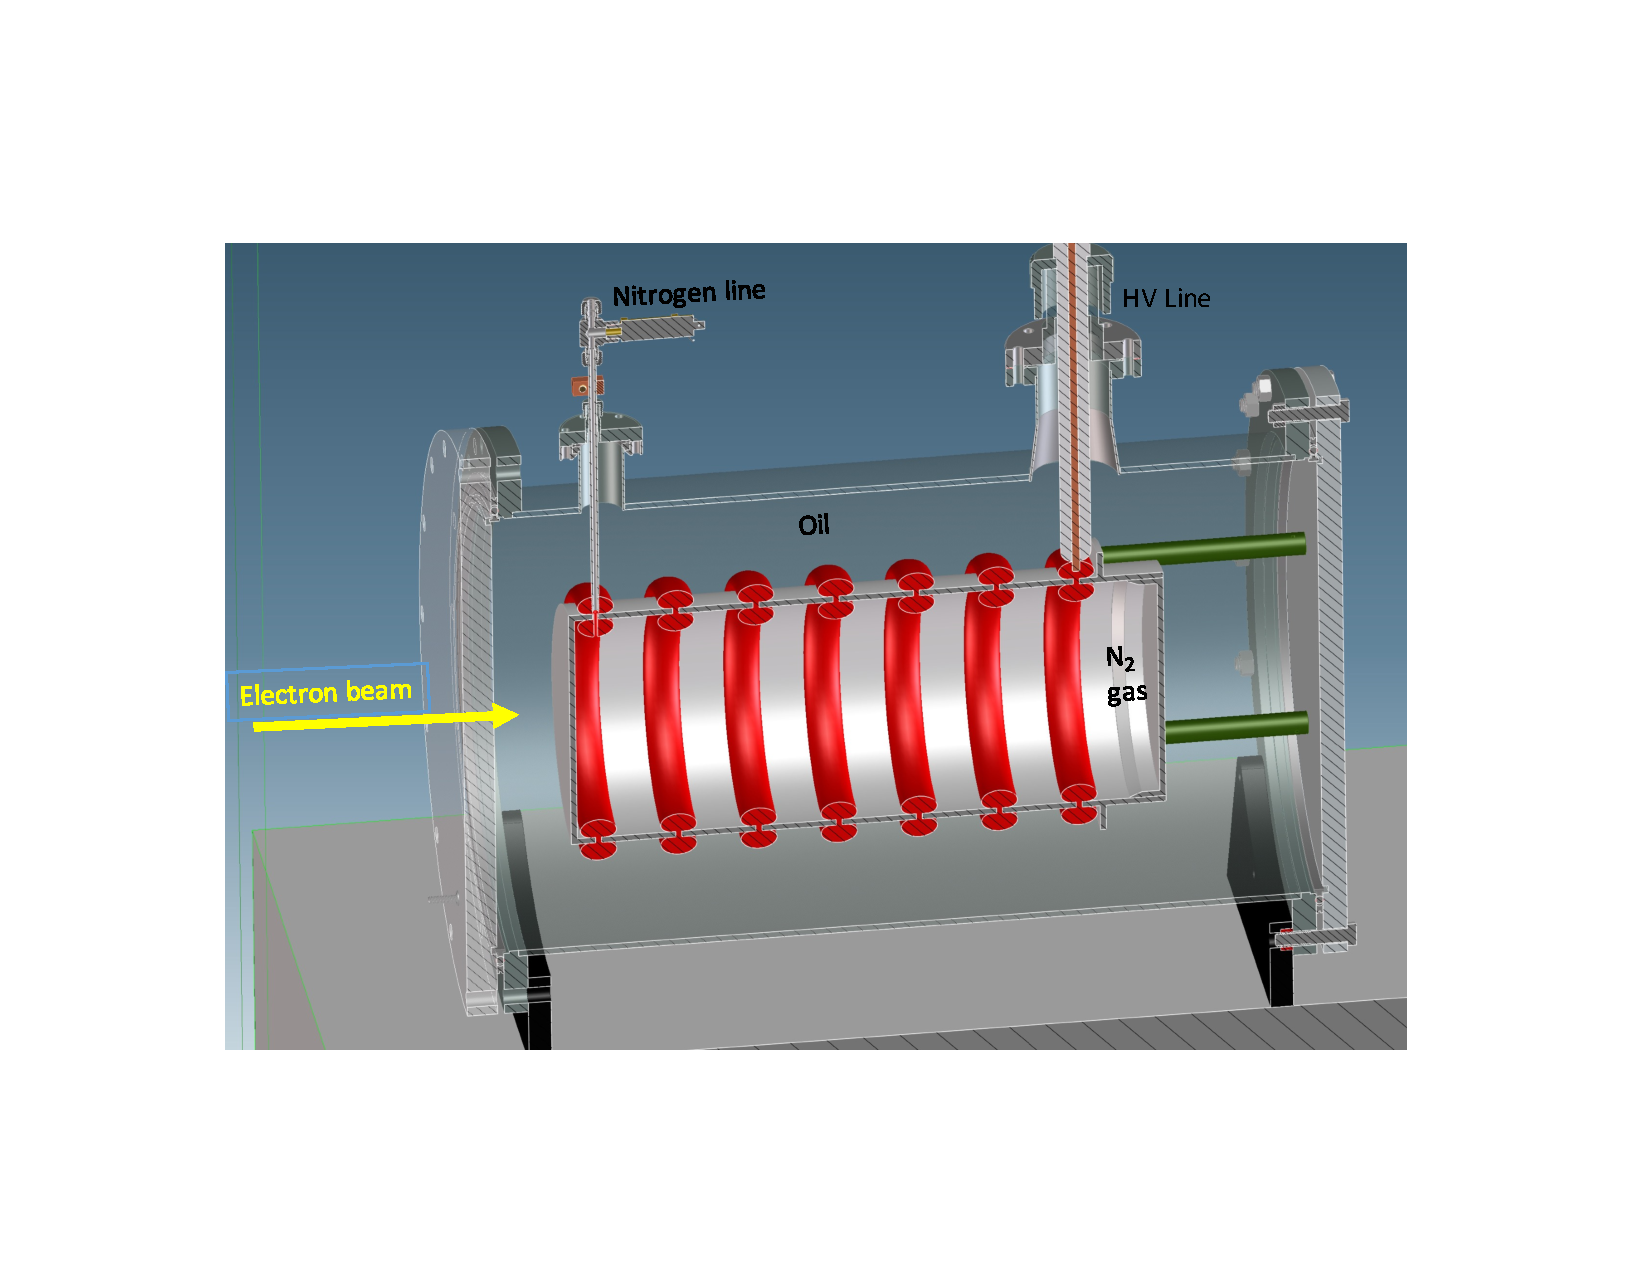
\includegraphics[width=0.8\textwidth]{beamwindow_SLACtest.pdf}
\end{cdrfigure}

\subsubsubsection{Full integration test in 35-ton cryostat}
Discuss field cage mock-up test.
\begin{cdrfigure}[PC4 Test setup]{beamwindow_PC4}{Field cage mock-up high voltage test in 35-ton (preliminary drawing).}
  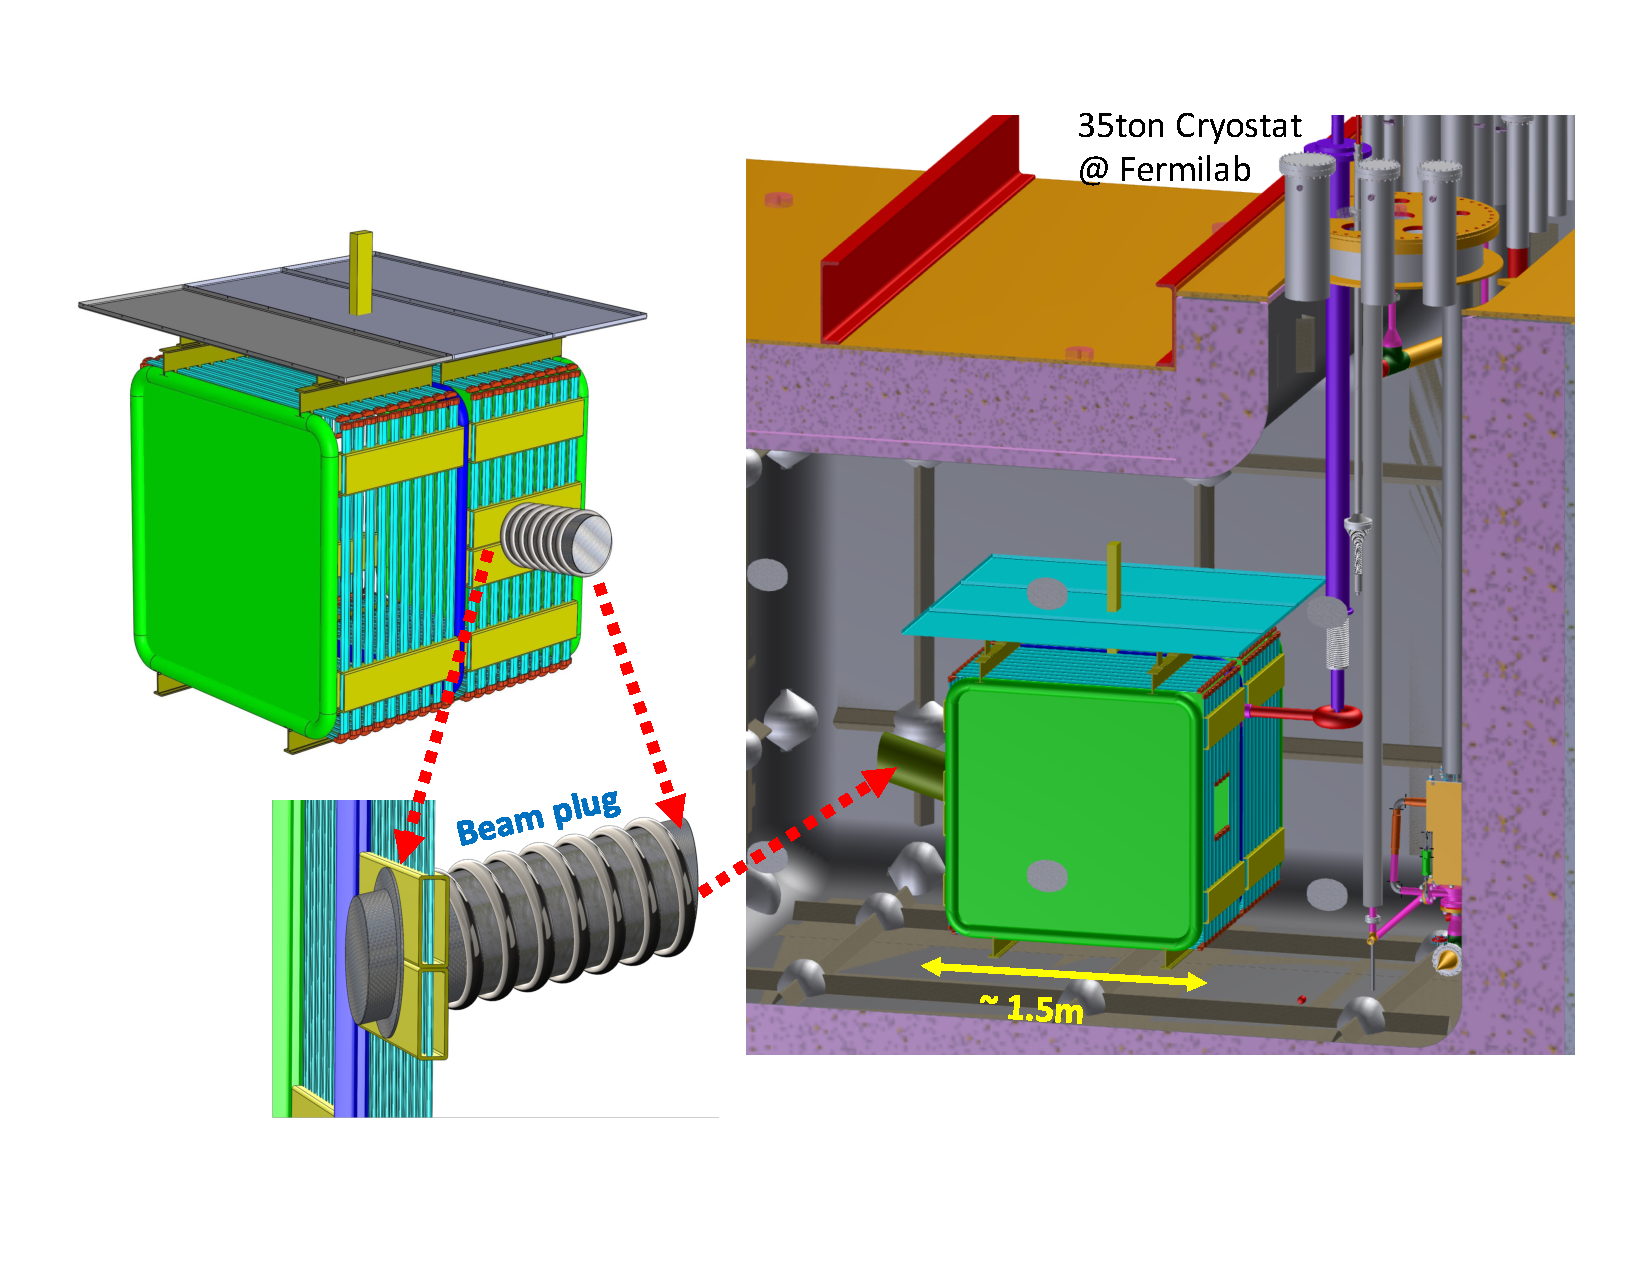
\includegraphics[width=0.95\textwidth]{beamwindow_PC4Test.pdf}
\end{cdrfigure}


